\documentclass[../engineering_mathematics_lecture_note.tex]{subfiles}
\begin{document}
\begin{definition}
    연립 상미분방정식은
    \begin{align*}
        y_1' &= f_1 (x, y_1, \dots, y_n)\\
             &\qquad\vdots \\
        y_n' &= f_n (x, y_1, \dots, y_n)
    \end{align*}
    와 같이 $y_1, \dots, y_n$에 대해 주어진 미분방정식들의 계를 의미한다.
    
    특히 위와 같이 1계 상미분방정식들의 계는 1계 연립 상미분방정식이라고 한다.
\end{definition}

\begin{example}
    1계 선형 연립 상미분방정식
    \begin{align*}
        y_1' &= a_{11} y_1 + \dots + a_{1n} y_n + b_1(x)\\
             &\phantom{= a_{11} y_1 + \dots} \vdots\\
        y_n' &= a_{n1} y_1 + \dots + a_{nn} y_n + b_n(x)
    \end{align*}
    을 행렬 표현으로 다시 정리하면
    \begin{equation*}
        \begin{pmatrix}
            y_1' \\ \vdots \\ y_n'
        \end{pmatrix}
        = \begin{pmatrix}
            a_{ij}
        \end{pmatrix}_{n \times n}
        \begin{pmatrix}
            y_1 \\ \vdots \\ y_n
        \end{pmatrix}
        + \begin{pmatrix}
            b_1 \\ \vdots \\ b_n
        \end{pmatrix}
    \end{equation*}
    이 되는데,
    \begin{equation*}
        \vec y =
        \begin{pmatrix}
            y_1 \\ \vdots \\ y_n
        \end{pmatrix}, \quad
        A = \begin{pmatrix}
            a_{ij}
        \end{pmatrix}_{n \times n}, \quad
        \vec b =
        \begin{pmatrix}
            b_1 \\ \vdots \\ b_n
        \end{pmatrix}
    \end{equation*}
    으로 두면
    \begin{equation*}
        \vec y' = A \vec y + \vec b
    \end{equation*}
    로 쓸 수 있다.
    만약 $\vec b = \vecz$라면 위 1계 선형 연립 상미분방정식은 제차이고, 그렇지 않은 경우 비제차이다.
\end{example}

\begin{theorem}
    제차 연립 상미분방정식 $\vec y' = A \vec y$에 대해서 $\vec y_1$과 $\vec y_2$가 해라면 일차결합 $c_1 \vec y_1 + c_2 \vec y_2$도 해이다.
\end{theorem}

\begin{theorem}
    비제차 연립 상미분방정식 $\vec y' = A \vec y + \vec b$의 해 $\vec y$는 제차 연립 상미분방정식 $\vec y' = A \vec y$의 해 $\vec y_h$와 특수해 $\vec y_p$의 합 $\vec y_h + \vec y_p$이다.
\end{theorem}

\begin{theorem}
    제차 연립 상미분방정식 $\vec y' = A \vec y$의 $n \times n$ 계수 행렬 $A$의 모든 성분이 연속이면 해공간의 차원은 $n$이다.
\end{theorem}

\begin{example}
    상수계수 제차 연립 1계 상미분방정식 $\vec y' = A \vec y$에 대해서, $\vec v$가 상수 벡터일 때
    \begin{equation*}
        \vec y = e^{tx} \vec v
    \end{equation*}
    를 대입한다:
    \begin{equation*}
        t e^{tx} \vec v = A e^{tx} \vec v
    \end{equation*}
    가 되고, 정리하면
    \begin{equation*}
        A \vec v = t \vec v
    \end{equation*}
    가 된다.
    따라서 $t$는 $A$의 특성값이며, $\vec v$는 $A$의 $t$-특성벡터이다.
\end{example}

\begin{example}
    상수계수 제차 연립 1계 상미분방정식
    \begin{equation*}
        \vec y' = \begin{pmatrix}
            -3 & 1 \\
            1 & -3
        \end{pmatrix}
        \vec y
    \end{equation*}
    이 주어졌을 때, 계수 행렬의 특성다항식 $\Char A$는
    \begin{equation*}
        \Char A = t^2 + 6t + 8
    \end{equation*}
    이므로 해는 $t = -2$ 혹은 $t = -4$ 이다.
    \begin{enumerate}
        \item $t = -2$인 경우
            \begin{equation*}
                A + 2I = \begin{pmatrix}
                    -1 & 1\\
                    1 & -1
                \end{pmatrix}
            \end{equation*}
            이므로 특성벡터는 $(1, 1)$ 이다.
        \item $t = -4$인 경우
            \begin{equation*}
                A + 4I = \begin{pmatrix}
                    1 & 1\\
                    1 & 1
                \end{pmatrix}
            \end{equation*}
            이므로 특성벡터는 $(1, -1)$ 이다.
    \end{enumerate}
    이제 특성값과 특성벡터를 통해 연립 상미분방정식의 두 해
    \begin{equation*}
        e^{-2x} \begin{pmatrix}
            1 \\ 1
        \end{pmatrix}, \quad e^{-4x} \begin{pmatrix}
            1 \\ -1
        \end{pmatrix}
    \end{equation*}
    을 구할 수 있다.
    따라서 일반해는
    \begin{equation*}
        \vec y = c_1 e^{-2x} \begin{pmatrix}
            1 \\ 1
        \end{pmatrix} + c_2 e^{-4x} \begin{pmatrix}
            1 \\ -1
        \end{pmatrix}
    \end{equation*}
    이므로
    \begin{align*}
        y_1 &= c_1 e^{-2x} + c_2 e^{-4x}\\
        y_2 &= c_1 e^{-2x} - c_2 e^{-4x}
    \end{align*}
    로 해를 구할 수 있다.

    만약 초기조건이 $\vec y(x_0) = \bigl(y_1(x_0), y_2(x_0) \bigr)$으로 주어졌다면,
    \begin{align*}
        c_1 e^{-2 x_0} + c_2 e^{-4 x_0} &= y_1(x_0)\\
        c_1 e^{-2 x_0} - c_2 e^{-4 x_0} &= y_2(x_0)
    \end{align*}
    이므로 항상 $c_1$과 $c_2$를 유일하게 결정할 수 있다.
\end{example}

지금까지의 예시에서 종속변수 $y$의 독립변수 $x$를 $t$로 표기하고, 특성값 $t$를 $\lambda$로 표기하자.
$\vec y$의 $t$에 따른 자취를 $y_1$-$y_2$ 평면에 그린 것을 상평면(phase portrait)라고 한다.

위의 예시에서처럼 특성값이 -2와 -4로 나오고, 그에 따른 특성벡터가 $(1, 1)$과 $(1, -1)$일 경우, 다음과 같은 상평면를 그릴 수 있다:
\begin{figure}[H]
    \centering
    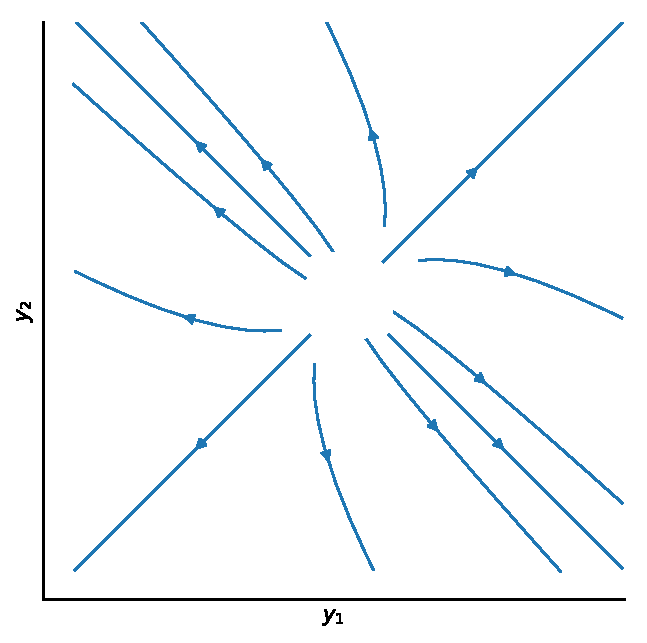
\includegraphics[width=0.5\linewidth]{plots/ex2.pdf}
    \label{fig:plots/ex2.pdf}
\end{figure}

특성값이 2와 5가 나오고, 특성벡터가 각각 $(1, 1)$과 $(1, -1)$로 나오면 다음과 같이 상평면를 그릴 수 있다:
\begin{figure}[H]
    \centering
    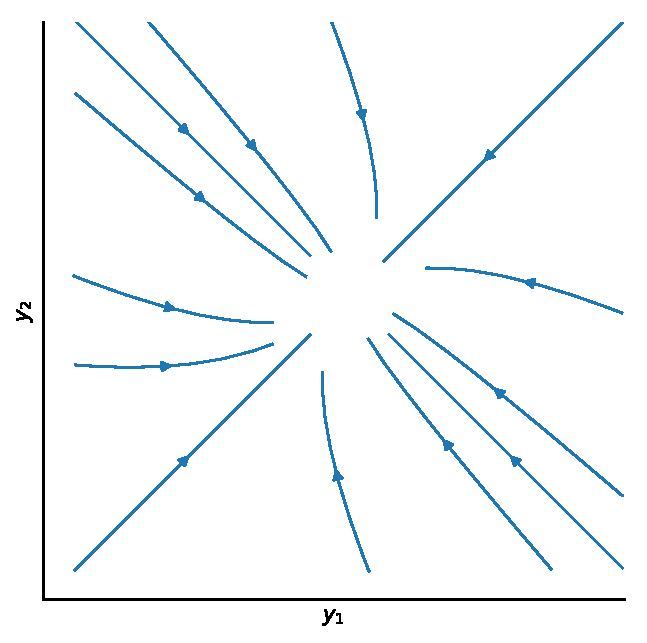
\includegraphics[width=0.5\linewidth]{plots/ex1.pdf}
    \label{fig:plots/ex1.pdf}
\end{figure}

상평면의 궤적은 해의 유일성에 따라 서로 교차하지 않는다.

일반적으로\marginpar{\small 2018.11.5} $\vec y' = A \vec y$의 연립 상미분방정식의 계수 행렬 $A$의 특성값이 $\lambda_1, \lambda_2$이고 각각 특성벡터 $\vec x_1$과 $\vec x_2$를 가질 때, 해를
\begin{equation*}
    \vec y(t) = c_1 e^{\lambda_1 t} \vec x_1 + c_2 e^{\lambda_2 t} \vec x_2
\end{equation*}
로 둘 수 있다.
이때 특성값의 분류에 따라 상평면이 어떻게 그려지는지 살펴본다.
\begin{enumerate}
    \item 서로 다른 $\lambda_1$과 $\lambda_2$가 같은 부호를 가질 때\\
        아래의 상평면에서 원점을 비고유마디점(improper node)이라고 한다.
        특히 아래의 경우에서는 해들이 중심으로 모이는 안정 평형점(stable equilibrium point)이다.
        \begin{figure}[H]
            \centering
            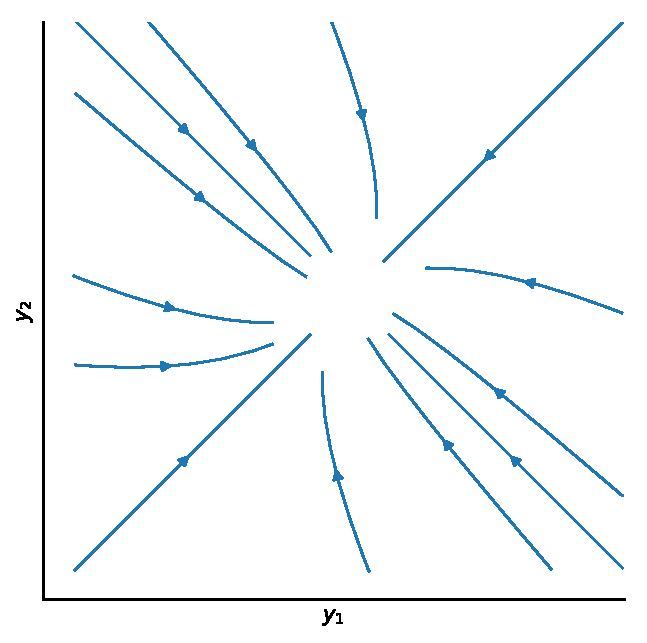
\includegraphics[width=0.5\linewidth]{plots/improper_node.pdf}
            \label{fig:plots/improper_node.pdf}
        \end{figure}
    \item $\lambda_1$과 $\lambda_2$가 서로 다른 부호를 가질 때 ($\lambda_1 < 0 < \lambda_2$)\\
        아래의 상평면에서 원점을 안장점(saddle point)이라고 한다.
        특히 아래의 경우에서는 해들이 중심에서 퍼지는 불안정 평형점(unstable equilibrium point)이다.
        \begin{figure}[H]
            \centering
            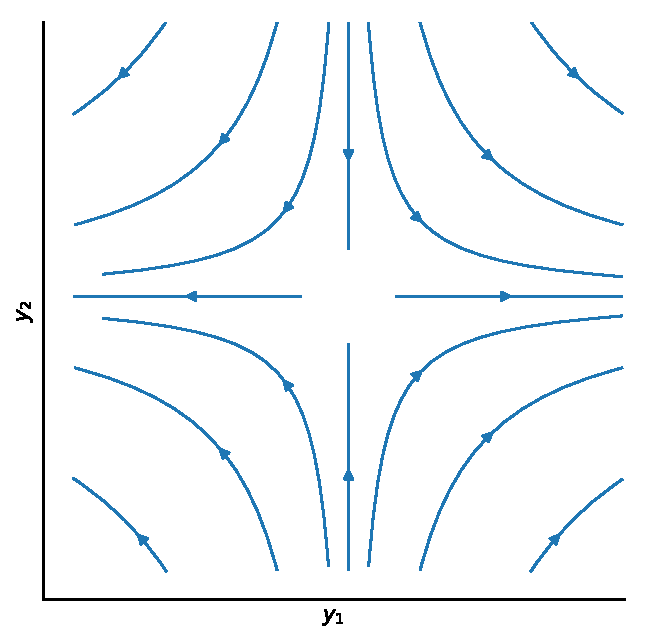
\includegraphics[width=0.5\linewidth]{plots/saddle_point.pdf}
            \label{fig:plots/saddle_point.pdf}
        \end{figure}
    \item $\lambda_1$과 $\lambda_2$가 같으면서 기하적 중복도가 2일 때\\
        $\lambda_1 = \lambda_2 = \lambda$라고 하자.
        기하적 중복도가 2이므로 $\left< \vec x_1, \vec x_2 \right> = \mathbb R^2$이며, $A$는 $\mathbb R^2$의 모든 벡터를 $\lambda$배하는 $\lambda I_{2 \times 2}$임을 알 수 있다.
        특성벡터를 표준기저벡터로 잡으면
        \begin{equation*}
            \vec y = e^{\lambda t} \left(c_1 \begin{pmatrix}
                1 \\ 0
            \end{pmatrix}
            + c_2 \begin{pmatrix}
                0 \\ 1
        \end{pmatrix}\right) = e^{\lambda t} \begin{pmatrix}
            c_1 \\ c_2
        \end{pmatrix}
        \end{equation*}
        이다.
        \begin{figure}[H]
            \centering
            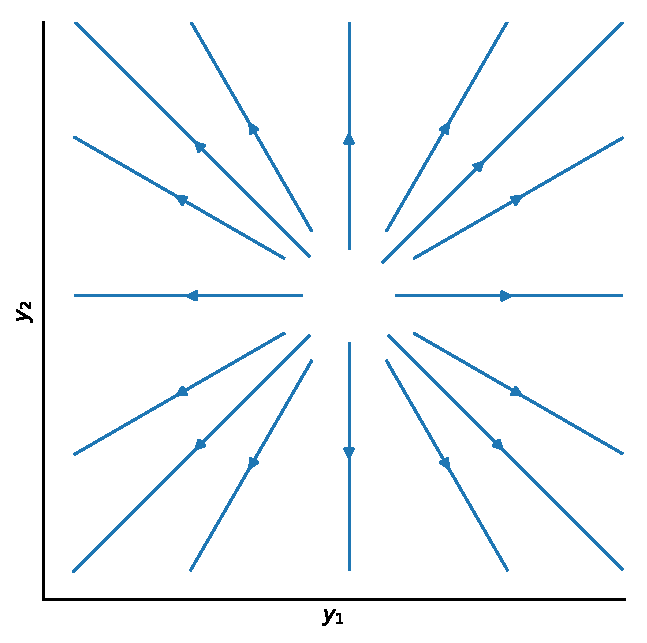
\includegraphics[width=0.5\linewidth]{plots/proper_node.pdf}
            \label{fig:plots/proper_node.pdf}
        \end{figure}
        위의 상평면에서 원점을 고유마디점(proper node)이라고 한다.
    \item $\lambda_1$과 $\lambda_2$가 같으면서 기하적 중복도가 1일 때\\
        $\lambda_1 = \lambda_2 = \lambda$라고 하자.
        기하적 중복도가 1이므로 특성벡터는 $\vec x$ 하나로 둘 수 있다.
        예를 들어, 연립 상미분방정식
        \begin{equation*}
            \vec y' = \begin{pmatrix}
                4 & 1\\
                -1 & 2
            \end{pmatrix}
            \vec y
        \end{equation*}
        의 특성다항식은
        \begin{equation*}
            (4 - \lambda)(2 - \lambda) + 1 = (\lambda - 3)^2
        \end{equation*}
        이 나와 특성값 3만을 가진다.
        \begin{equation*}
            A - 3I = \begin{pmatrix}
                1 & 1\\
                -1 & -1
            \end{pmatrix}
        \end{equation*}
        이므로 특성벡터 $\vec x = (1, -1)$로 둘 수 있다.
        따라서 한 해는
        \begin{equation*}
            e^{3t} \begin{pmatrix}
                1 \\ -1
            \end{pmatrix}
        \end{equation*}
        이다.
        어떤 벡터 $\vec u$에 대해 새로운 해를
        \begin{equation*}
            e^{3t} \left( t \begin{pmatrix}
                1 \\ -1
        \end{pmatrix} + \vec u\right)
        \end{equation*}
        로 두고\footnote{이러한 벡터 $\vec u$는 유일하게 존재함이 알려져 있다.} 위 연립 상미분방정식에 대입하면
        \begin{equation*}
            e^{3t} \left( \begin{pmatrix}
                1 \\ -1
            \end{pmatrix} + 3t \begin{pmatrix}
                1 \\ -1
            \end{pmatrix} + \vec u \right) = e^{3t} \begin{pmatrix}
            4 & 1\\
            -1 & 2
            \end{pmatrix}
            \left( t \begin{pmatrix}
                1 \\ -1
        \end{pmatrix} + \vec u \right)
        \end{equation*}
        가 된다.
        정리하면
        \begin{equation*}
            \begin{pmatrix}
                1 \\ -1
                \end{pmatrix}+ \vec u = \begin{pmatrix}
                4 & 1 \\
                -1 & 2
            \end{pmatrix} \vec u
        \end{equation*}
        가 되어
        \begin{equation*}
            \begin{pmatrix}
                3 & 1\\
                -1 & 1
            \end{pmatrix} \vec u = \begin{pmatrix}
                1 \\ -1
            \end{pmatrix}
        \end{equation*}
        이 된다.
        따라서 역함수를 계산한 후 정리하면
        \begin{equation*}
            \vec u = \frac14 \begin{pmatrix}
                1 & -1\\
                1 & 3
            \end{pmatrix} \begin{pmatrix}
                1 \\ -1
            \end{pmatrix} = \begin{pmatrix}
            \frac12 \\ -\frac12
            \end{pmatrix}
        \end{equation*}
        그러므로 일반해 $\vec y$는
        \begin{equation*}
            \vec y = c_1 e^{3t} \begin{pmatrix}
                1 \\ -1
            \end{pmatrix} + c_2 e^{3t} \left( t \begin{pmatrix}
                1 \\ -1
            \end{pmatrix}  + \begin{pmatrix}
                \frac12 \\ -\frac12
        \end{pmatrix}\right)
        \end{equation*}
        임을 알 수 있다.
        \begin{figure}[H]
            \centering
            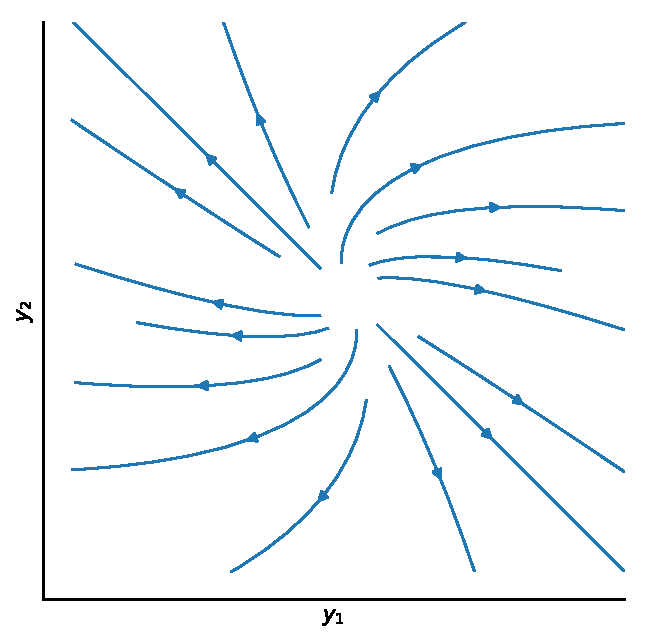
\includegraphics[width=0.5\linewidth]{plots/degenerate_node.pdf}
            \label{fig:plots/degenerate_node.pdf}
        \end{figure}
        위의 상평면에서 원점을 퇴화마디점(degenerate node)이라고 한다. 
    \item $\lambda_1$과 $\lambda_2$가 서로 다른 순허수일 때\\
        $\lambda_1 = ai, \lambda_2 = -ai$라고 하자.\footnote{연립 상미분방정식의 계수 행렬이 실행렬이므로 그 특성다항식의 복소해가 켤레로 나타난다.}
        $\lambda_1$-특성벡터를 $\tilde{\vec x}_1$, $\lambda_2$-특성벡터를 $\tilde{\vec x}_2$라고 하자.
        그러면 $\tilde{\vec x}_1$과 $\tilde{\vec x}_2$도 서로 켤레이고, 복소해 $\tilde{\vec y}$는
        \begin{equation*}
            \tilde{\vec y} = c_1 e^{ait} \tilde{\vec x}_1 + c_2 e^{-ait} \tilde{\vec x}_2
        \end{equation*}
        로 나타낼 수 있다.
        그러나 실근을 찾고자 한다면, 서로 켤레인
        \begin{equation*}
            e^{ait} \tilde{\vec x}_1, \qquad e^{ait} \tilde{\vec x}_2
        \end{equation*}
        의 합과 차를 사용해
        \begin{equation*}
            \frac{e^{ait} \tilde{\vec x}_1 + e^{-ait} \tilde{\vec x}_2}{2}, \quad \frac{e^{ait} \tilde{\vec x}_1 - e^{-ait} \tilde{\vec x}_2}{2i}
        \end{equation*}
        의 두 실근을 찾을 수 있다.
        따라서 실수 일반해 $\vec y$는
        \begin{equation*}
            \vec y = c_1 \frac{e^{ait} \tilde{\vec x}_1 + e^{-ait} \tilde{\vec x}_2}{2} + c_2 \frac{e^{ait} \tilde{\vec x}_1 - e^{-ait} \tilde{\vec x}_2}{2i}
        \end{equation*}
        로 쓸 수 있다.
        
        예를 들어 연립 상미분방정식
        \begin{equation*}
            \vec y' = \begin{pmatrix}
                0 & 1\\
                -4 & 0
            \end{pmatrix}
            \vec y
        \end{equation*}
        에서 계수 행렬의 특성다항식은
        \begin{equation*}
            \lambda^2 + 4 = 0
        \end{equation*}
        이다.
        따라서 해는 $\lambda = \pm 2i$가 되고,
        \begin{equation*}
            \left( \begin{pmatrix}
                0 & 1\\
                -4 & 0
            \end{pmatrix}
            - 2i \begin{pmatrix}
                1 & 0\\
                0 & 1
            \end{pmatrix} \right) \begin{pmatrix}
                x \\ y
            \end{pmatrix}
            = \begin{pmatrix}
                -2i & 1\\
                -4 & -2i
            \end{pmatrix}
            \begin{pmatrix}
                x \\ y
            \end{pmatrix}
            = \begin{pmatrix}
                0 \\ 0
            \end{pmatrix}
        \end{equation*}
        이므로 $2i$-특성벡터 $\tilde{\vec x}_1$은 $(1, 2i)$이고, $-2i$-특성벡터 $\tilde{\vec x}_2$는 그 켤레인 $(1, -2i)$가 된다.
        따라서 복소해는
        \begin{equation*}
            e^{2it} \begin{pmatrix}
                1 \\ 2i
                \end{pmatrix}, \qquad e^{-2it} \begin{pmatrix}
                1 \\ -2i
            \end{pmatrix}
        \end{equation*}
        인데, 삼각함수를 통해
        \begin{equation*}
            \begin{pmatrix}
                \cos 2t + i \sin 2t\\
                2i(\cos 2t + i \sin 2t)
            \end{pmatrix}, \qquad \begin{pmatrix}
                \cos 2t - i \sin 2t\\
                -2i (\cos 2t - i \sin 2t)
            \end{pmatrix}
        \end{equation*}
        로 쓸 수 있다.
        따라서 합과 차를 통해 실수해
        \begin{equation*}
            \begin{pmatrix}
                \cos 2t\\
                -2 \sin 2t
            \end{pmatrix}, \qquad \begin{pmatrix}
                \sin 2t\\
                2\cos 2t
            \end{pmatrix}
        \end{equation*}
        를 구할 수 있다.
        그러므로 일반해 $\vec y$는
        \begin{align*}
            \vec y &= c_1 \begin{pmatrix}
                \cos 2t\\ -2 \sin 2t
            \end{pmatrix} + c_2 \begin{pmatrix}
                \sin 2t\\ 2 \cos 2t
            \end{pmatrix}\\
                   &= c_1 \begin{pmatrix}
                \cos 2t\\ -2 \sin 2t
            \end{pmatrix} + c_2 \begin{pmatrix}
            \cos \left( \frac{\pi}{2} - 2t \right)\\ 2 \sin \left( \frac{\pi}{2} -2t \right)
        \end{pmatrix}
        \end{align*}
        가 된다.

        \begin{figure}[H]
            \centering
            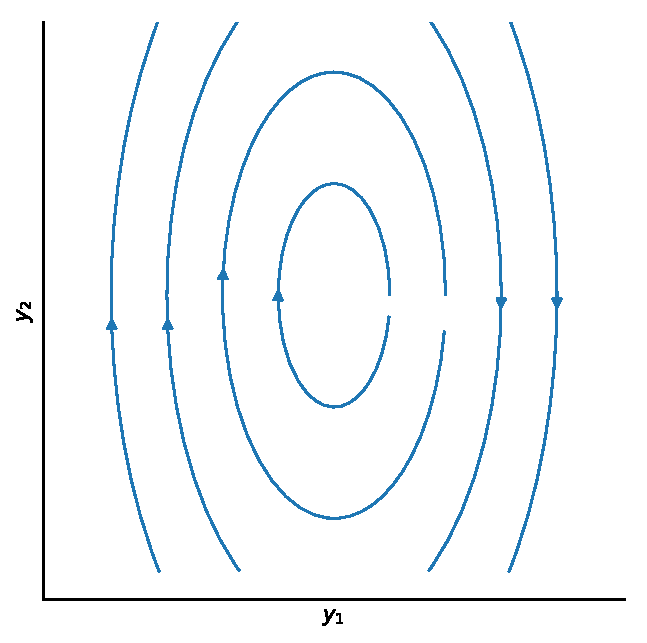
\includegraphics[width=0.5\linewidth]{plots/center.pdf}
            \label{fig:plots/center.pdf}
        \end{figure}
        위의 상평면에서 원점을 중심점(center)이라고 한다. 
    \item $\lambda_1$과 $\lambda_2$가 서로 다른 순허수나 실수가 아닌 복소수일 때\\
        $\lambda_1 = a + bi$, $\lambda_2 = a - bi$로 두자.
        예를 들어,
        \begin{equation*}
            \vec y' = \begin{pmatrix}
                -1 & 1\\
                -1 & -1
            \end{pmatrix}
            \vec y
        \end{equation*}
        의 연립 상미분방정식에서 계수 행렬의 특성다항식은
        \begin{equation*}
            \lambda^2 + 2\lambda _2 = 0
        \end{equation*}
        이고, 해는 $\lambda = -1 \pm i$이다.
        두 복소해를 조합해 실수해를 구하면
        \begin{equation*}
            e^{-t} \begin{pmatrix}
                \cos t\\ -\sin t
                \end{pmatrix},\qquad e^{-t} \begin{pmatrix}
                \sin t \\ \cos t
            \end{pmatrix}
        \end{equation*}
        가 된다.
        따라서 일반해 $\vec y$는
        \begin{equation*}
            \vec y = e^{-t} \left( c_1 \begin{pmatrix}
                \cos t\\ -\sin t
            \end{pmatrix} + c_2 \begin{pmatrix}
                \sin t \\ \cos t
            \end{pmatrix} \right)
        \end{equation*}
        로 쓸 수 있다.
        \begin{figure}[H]
            \centering
            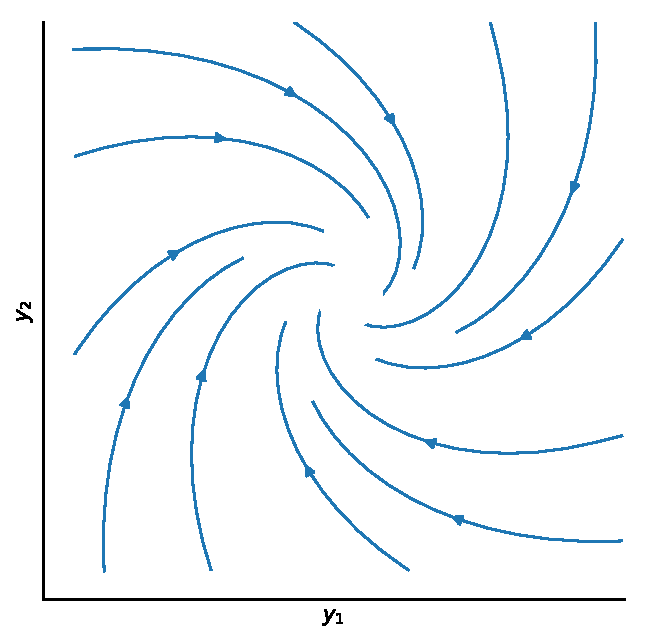
\includegraphics[width=0.5\linewidth]{plots/spiral_point.pdf}
            \label{fig:plots/spiral_point.pdf}
        \end{figure}
        위의 상평면에서 원점을 나선점(spiral point)이라고 한다. 
\end{enumerate}
\end{document}
